Dette kapitel evaluerer de to valgte sensormodeller(\cref{mapping:sensormodel}) og ruteplanlægning(\cref{ruteplanleagning}).


\section{Formål}
Formålet med denne test er at se hvilken sensormodel der kommer frem til det mest præcise kort og hvilken indvirkning ruteplanlægningen har.

\section{Test}\label{evaluering:test_beskrivelse}
Der bliver foretaget tre tests med hver sensormodel(\cref{mapping:sensormodel}).
I alle test benyttes ruteplanlægning beskrevet i \cref{ruteplanlaegning}.
Startpositionen er altid den samme.
Robotten kører hen til et punkt og scanner to gange - dette foretages 75 gange.
Alle data bliver logget så det er muligt at genskabe et kort udfra det.

\begin{figure}
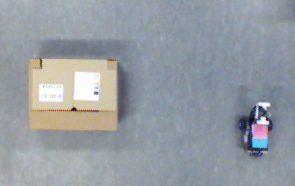
\includegraphics[width=\textwidth]{emptyGrid}
\label{evaluering:emptyGrid}
\caption{Forsøgsopstillingen inden hver test sættes i gang.}
\end{figure}

\subsection{Opstilling}

\subsection{Resultater}

\subsection{Opsummering}